\documentclass[12pt, times new roman]{article}
\usepackage[utf8]{inputenc}
\usepackage{graphicx}

\title{Profile Mahasiswa}
\author{Heriyanto}
\date{December 2019}

\begin{document}

\maketitle
\section{Membuat aplikasi melalui apex.oracle}
\subsection{Apex Oracle}
Application Express(Oracle Apex), dulu di sebut HTTP DB adalah sebuah Aplikasi database berbasis web yang digunakan dalam database Oracle. Oracle Apex ini mudah dipakai hanya menggunakan web browser saja dan proses pemrograman yang sederhana, serta mengembangkan ilmu dan kemampuan dengan Aplikasi ini secara aman dan cepat. Oracle Application Express memiliki kualitas database yang bagus, produktivitas dan standart luas yang dimiliki oleh perusahaan-perusahaan besar dan memiliki keamanan, stabilitas, ketersediaan dalam membangun suatu web. Application Express adalah suatu alat yang digunakan untuk membangun Aplikasi web-based. Selain itu Oracle Application Express tidak membutuhkan perangkat lainnya untuk mengembangkan, menyebarkan serta menjalankan Aplikasi, karena di dalam Oracle Application Express telah menyediakan tiga alat utama. Tiga alat utama ini memiliki Kegunaan yang penting di dalam Oracle Application Express:
\begin{itemize}
\item Application Builder : Membuat aplikasi, melihat aplikasi, mengimport aplikasi, mengatur service, mengatur user aplikasi dan memantau aktifitas yang di lakukan pengguna.
\item SQL Workshop : Membuat tabel dan komponennya (menggunakan kode PL-SQL secara manual maupun otomatis), melihat struktur tabel dan komponennya, mengimpor dan mengekspor script.
\item Utilitas : melihat report table dan komponennya dan history aplikasi.
\end{itemize}
\section{Langkah - Langkah Membuat Aplikasi di Apex Oracle}
\begin{enumerate}
\item Pertama login ke apex.oracle.com, lalu klik Sign in
\item Akan dialihkan ke halaman login application express, silahkan masuk untuk pengguna yang telah memiliki workspace, jika belum memiliki wokspace silahkan klik "Request a Workspace".
\begin{figure}[!htbp]
	\centering
	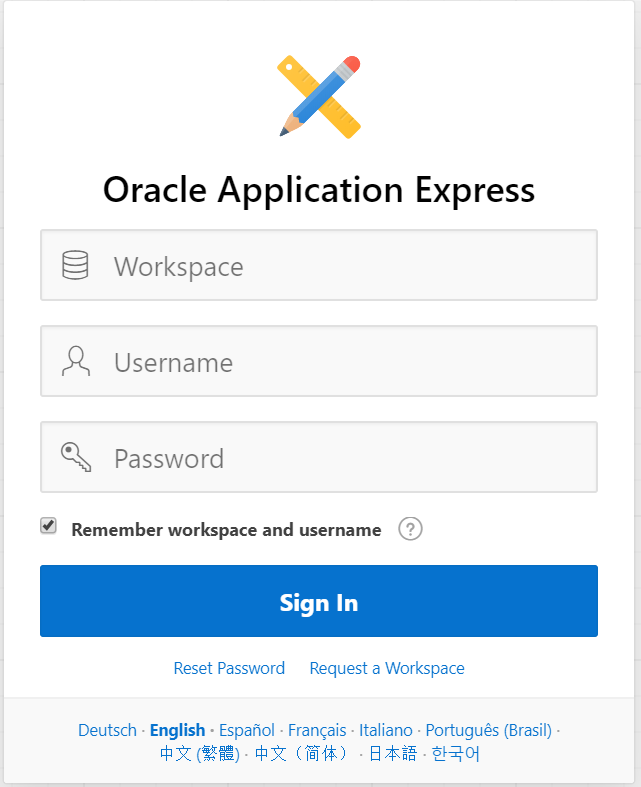
\includegraphics[width=5cm]{figures/17.png}
	\end{figure}
\item Cara membuat workspace cukup mudah, silahkan isi form yang telah disediakan setelah meminta workspace, lalu ikuti arahan selanjutnya.
\begin{figure}[!htbp]
	\centering
	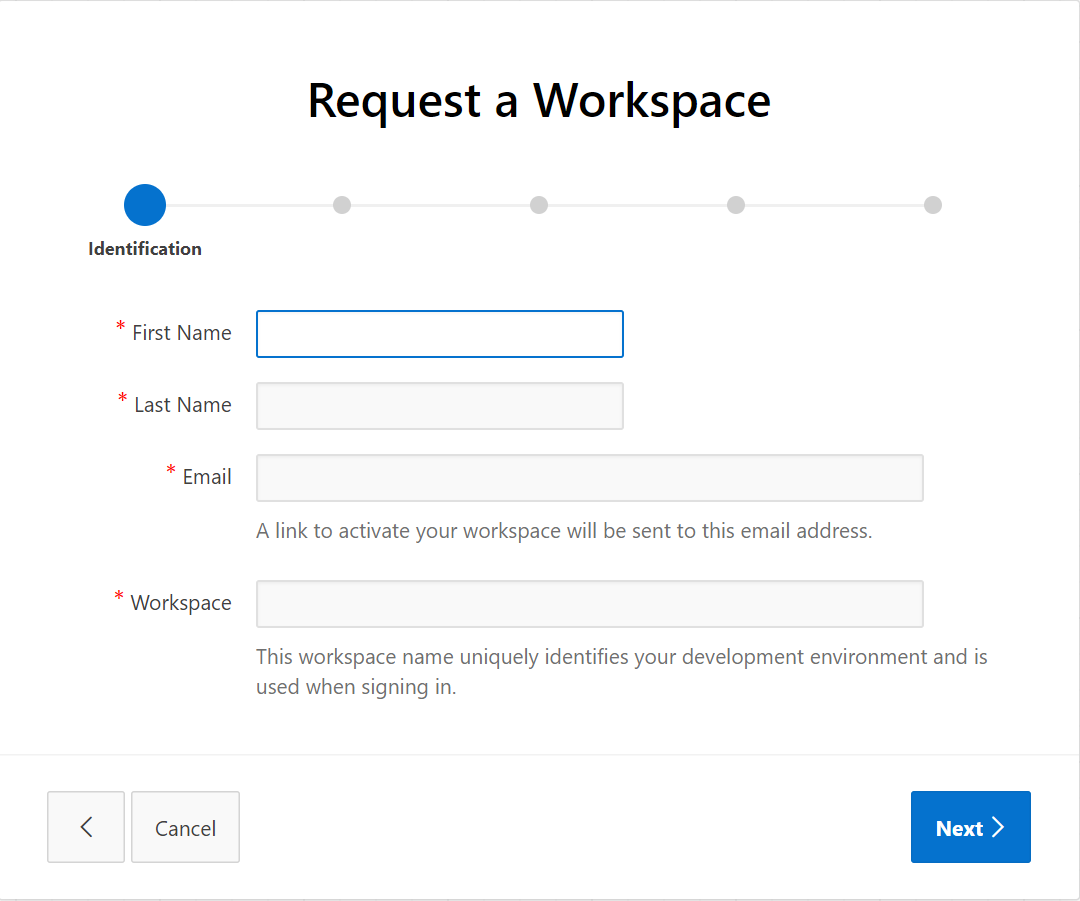
\includegraphics[width=6cm]{figures/18.png}
\end{figure}
\item Jika telah memiliki workspace silahkan login dengan menggunakan workspace tersebut dan username dan password yang anda buat.
\item Setelah login, di halaman utama klik "SQL Workshop", lalu pilih dan klik "SQL Commands".
\item Di SQL Commands ini kita akan membuat tabel terlebih dahulu. Tabel pertama adalah Tabel Mahasiswa. Ikuti sintaks dibawah:
\begin{figure}[!htbp]
	\centering
	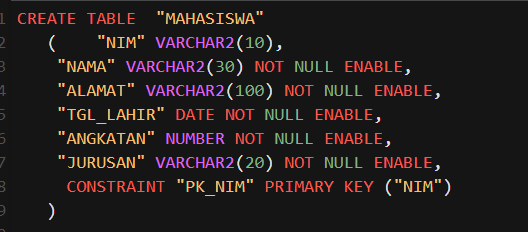
\includegraphics[width=10cm]{figures/1.png}
\end{figure}
\item Tabel selanjutnya adalah Tabel Matkul.
\begin{figure}[!htbp]
	\centering
	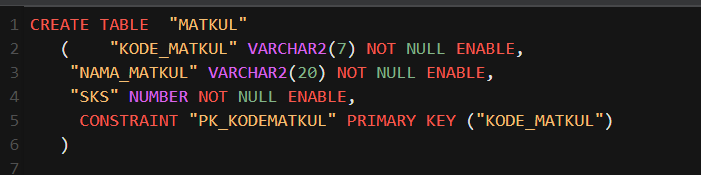
\includegraphics[width=10cm]{figures/2.png}
\end{figure}
\item Tabel ketiga adalah tabel Nilaimhs.
\begin{figure}[!htbp]
	\centering
	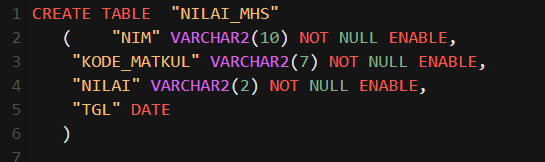
\includegraphics[width=10cm]{figures/3.png}
\end{figure}
\item Terakhir adalah tabel Logmhs.
\begin{figure}[!htbp]
	\centering
	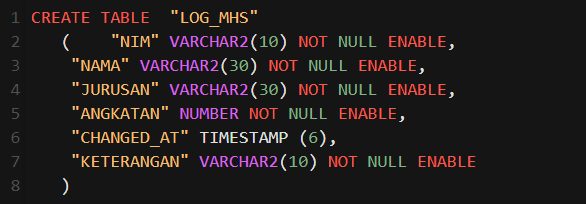
\includegraphics[width=10cm]{figures/4.png}
\end{figure}
\item Setelah semua tabel telah dibuat, sekarang kita akan membuat trigger. Trigger adalah blok PL/SQL yang disimpan dalam database dan akan diaktivasi ketika kita melakukan statement-statement SQL (DELETE, UPDATE, dan INSERT) pada sebuah tabel. Aktivasi trigger didasarkan pada event yang terjadi di dalam tabel tersebut sehingga trigger dapat membantu dalam menjaga integritas dan konsistensi data. Implementasi trigger yang sering ditemui dalam dunia nyata adalah untuk meng-set dan mengubah nilai kolom dalam suatu tabel sehingga validasi nilai dari tabel tersebut akan terjaga. Adanya trigger dalam database akan meringankan kita dalam pembuatan aplikasi karena di dalam aplikasi yang kita buat, kita tidak perlu lagi untuk melakukan validasi data.
\item Disini kita akan membuat after insert dan before insert. Pertama mari kita buat trigger after delete, ikuti sintaks dibawah:
\begin{figure}[!htbp]
	\centering
	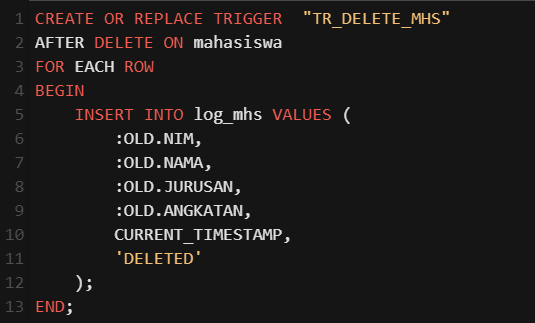
\includegraphics[width=10cm]{figures/8.png}
\end{figure}
\item Sekarang kita akan memasukkan data ke tabel-tabel tersebut secara manual, kecuali tabel logmhs yang datanya akan masuk secara otomatis karena trigger after insert yang telah kita buat tadi. Ketika ada perubahan data pada tabel mahasiswa akan langsung dimasukkan ke tabel logmhs. Sekarang kita coba menambah data di tabel mahasiswa.
\begin{figure}[!htbp]
	\centering
	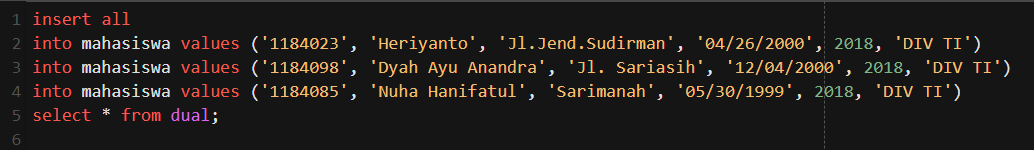
\includegraphics[width=10cm]{figures/5.png}
\end{figure}
\item Bisa dilihat dibawah bahwa data di logmhs telah ditambahkan setelah menambahkan data di tabel mahasiswa.
\begin{figure}[!htbp]
	\centering
	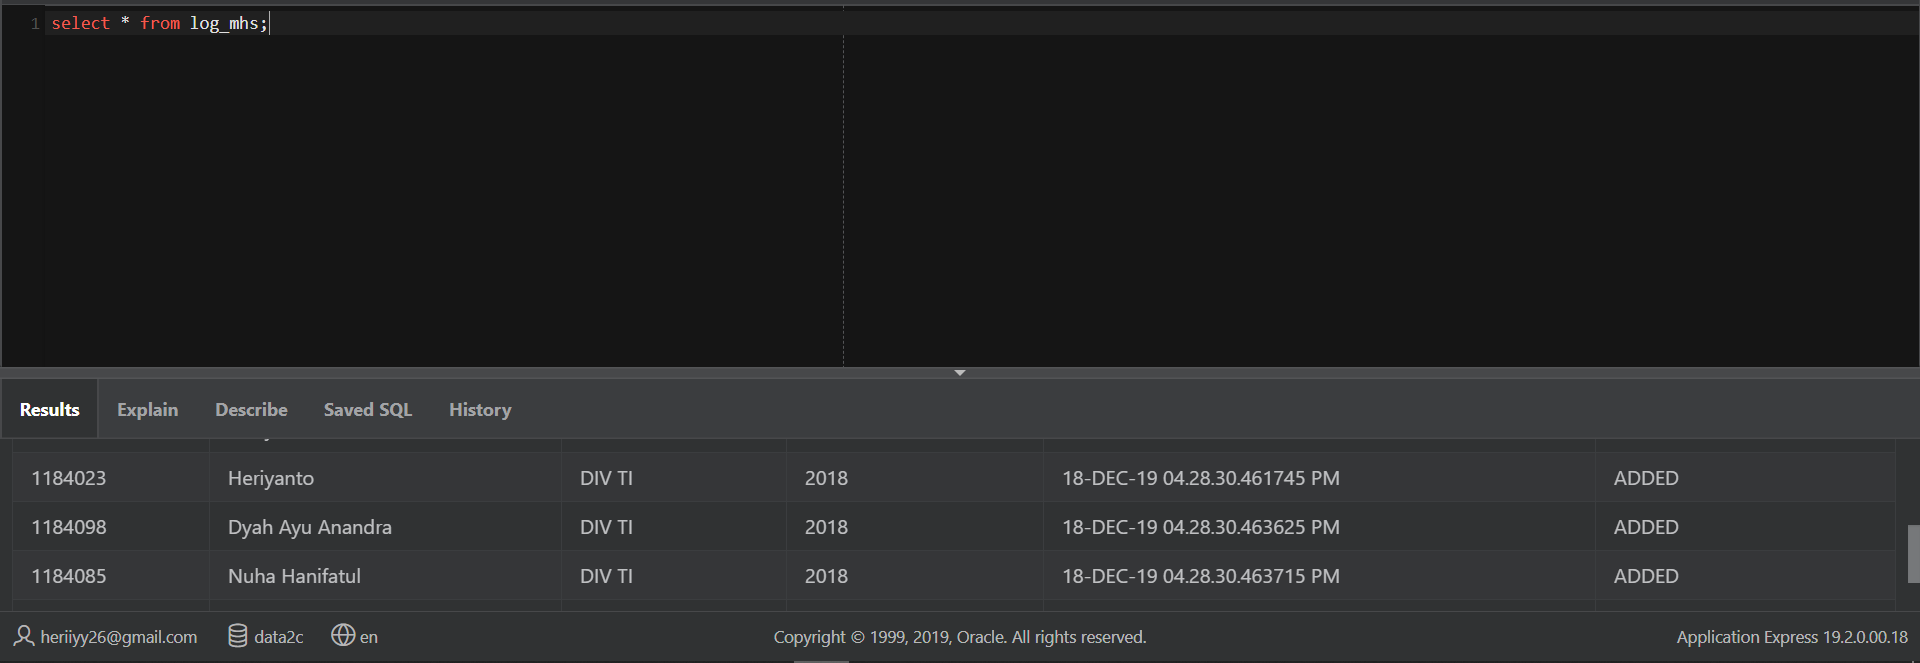
\includegraphics[width=10cm]{figures/20.png}
\end{figure}
\item Tak lupa untuk memasukkan data di tabel matkul.
\begin{figure}[!htbp]
	\centering
	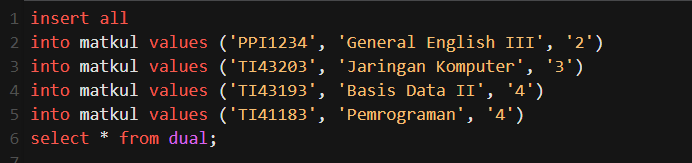
\includegraphics[width=10cm]{figures/6.png}
\end{figure}
\item Selanjutnya adalah membuat trigger before insert pada tabel nilaimhs.
\begin{figure}[!htbp]
	\centering
	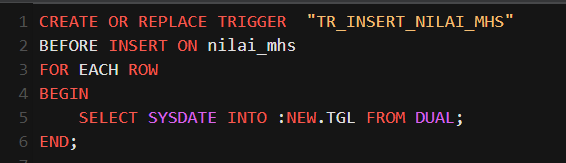
\includegraphics[width=10cm]{figures/19.png}
\end{figure}
\item Sekarang kita akan memasukkan data ke tabel nilaimhs tapi hanya untuk kolom nim, kodematkul, dan nilai saja. Kenapa tgl tidak, itu karena kita telah sebelumnya membuat trigger, kolom tgl akan terisi otomatis. Coba kita tambahkan data.
\begin{figure}[!htbp]
	\centering
	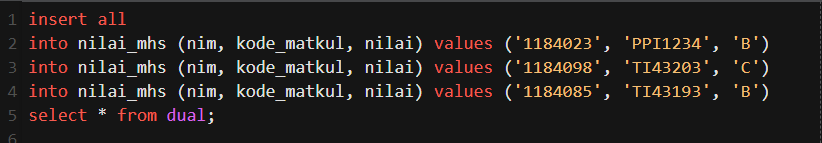
\includegraphics[width=10cm]{figures/7.png}
\end{figure}
\item Kita lihat bahwa trigger-nya berhasil, kolom tgl terisi dengan hari bulan dan tahun kita menambahkan data.
\begin{figure}[!htbp]
	\centering
	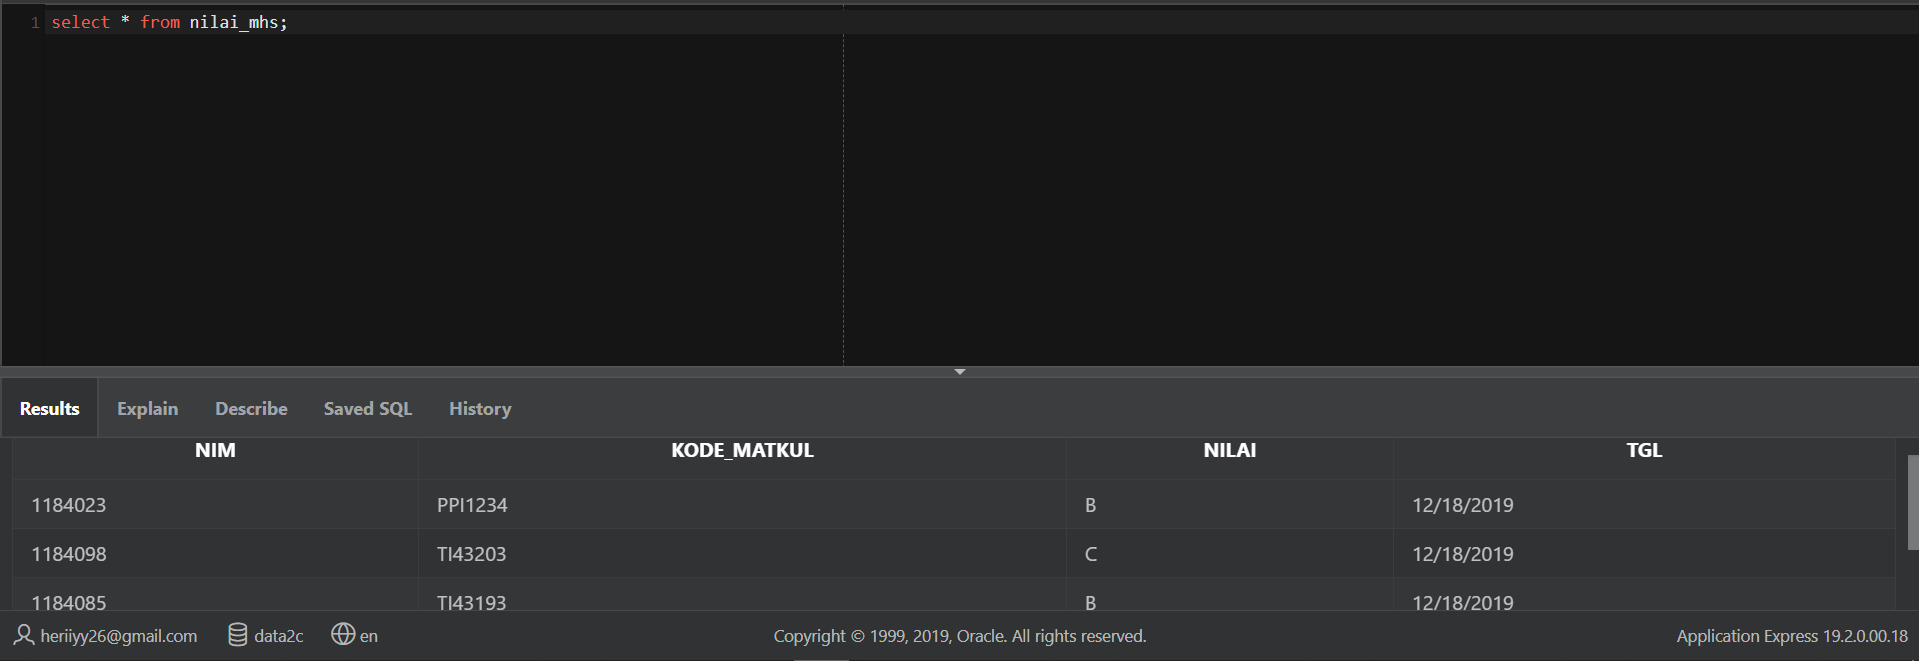
\includegraphics[width=12cm]{figures/21.png}
\end{figure}
\item Sekarang kita akan membuat view untuk table nilaimhs dimana akan menampilkan nim = 1184023. View dapat didefenisikan sebagai ‘tabel virtual’. Tabel ini bisa berasal dari tabel lain, atau gabungan dari beberapa tabel. Tujuan dari pembuatan VIEW adalah untuk kenyamanan (mempermudah penulisan query), untuk keamanan (menyembunyikan beberapa kolom yang bersifat rahasia), atau dalam beberapa kasus bisa digunakan untuk mempercepat proses menampilkan data (terutama jika kita akan menjalankan query tersebut secara berulang).
\begin{figure}[!htbp]
	\centering
	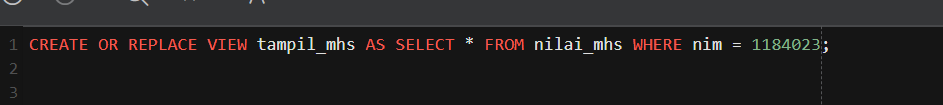
\includegraphics[width=12cm]{figures/11.png}
\end{figure}
\item Untuk melihat hasil dari view dengan cara select * from nama view.
\begin{figure}[!htbp]
	\centering
	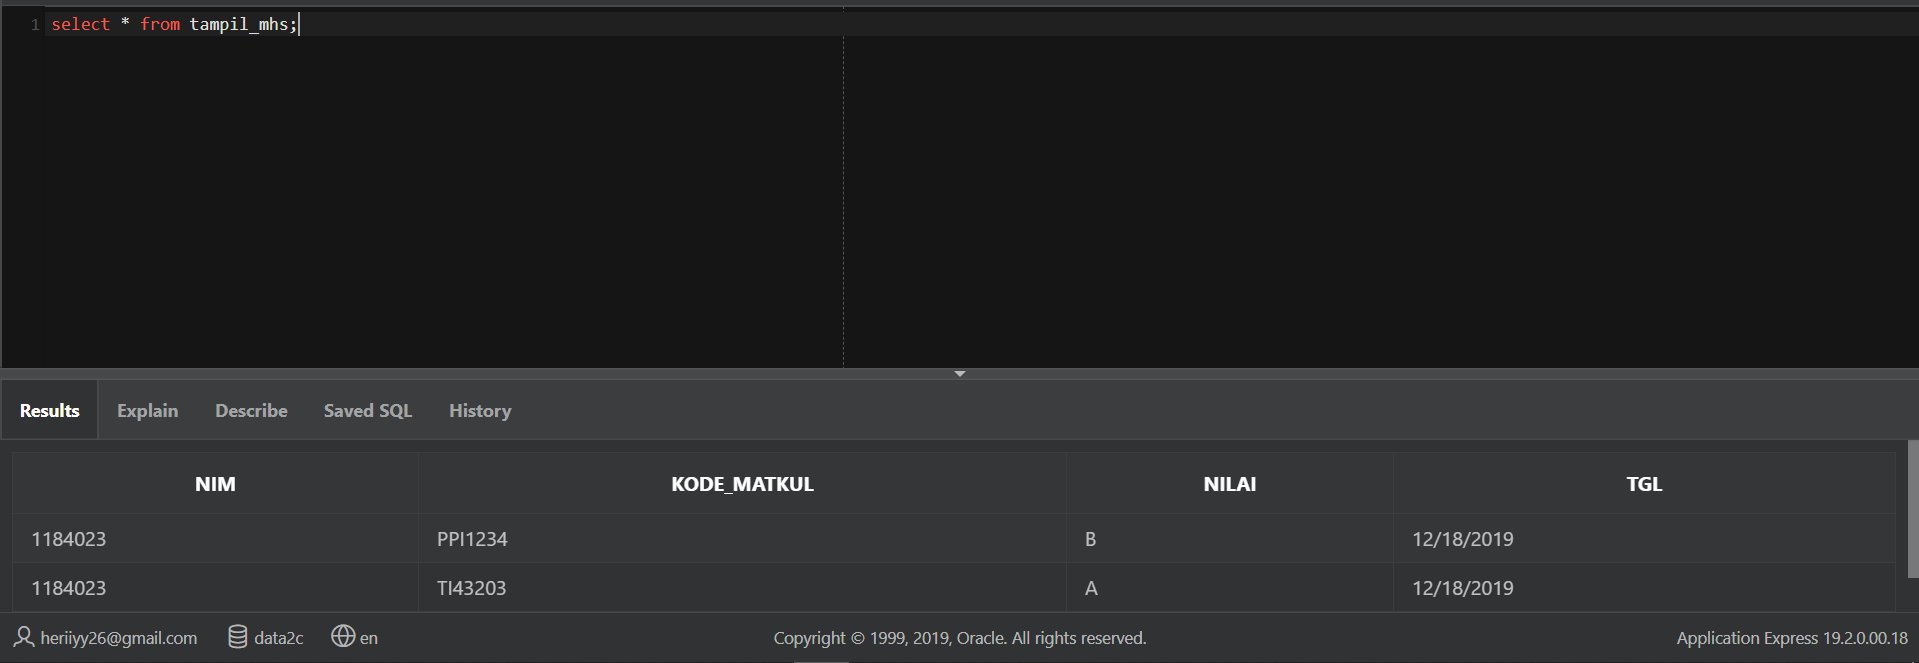
\includegraphics[width=10cm]{figures/22.png}
\end{figure}
\item Selanjutnya pembuatan aplikasi Profile Mahasiswa. Caranya adalah klik "App Builder" lalu klik "Create".
\item Setelah itu pilih "New Application".
\begin{figure}[!htbp]
	\centering
	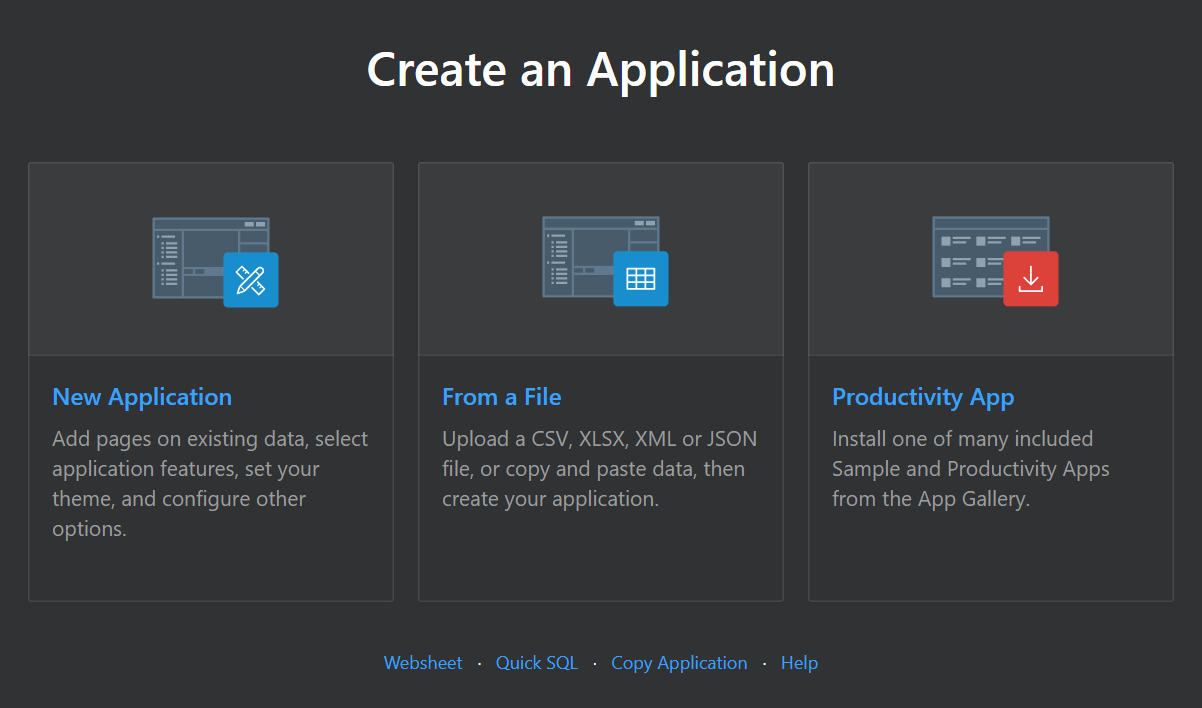
\includegraphics[width=9cm]{figures/27.png}
\end{figure}
\item Lalu isi form nama aplikasi dan tambahkan menu pada aplikasi dengan klik "Add Page".
\begin{figure}[!htbp]
	\centering
	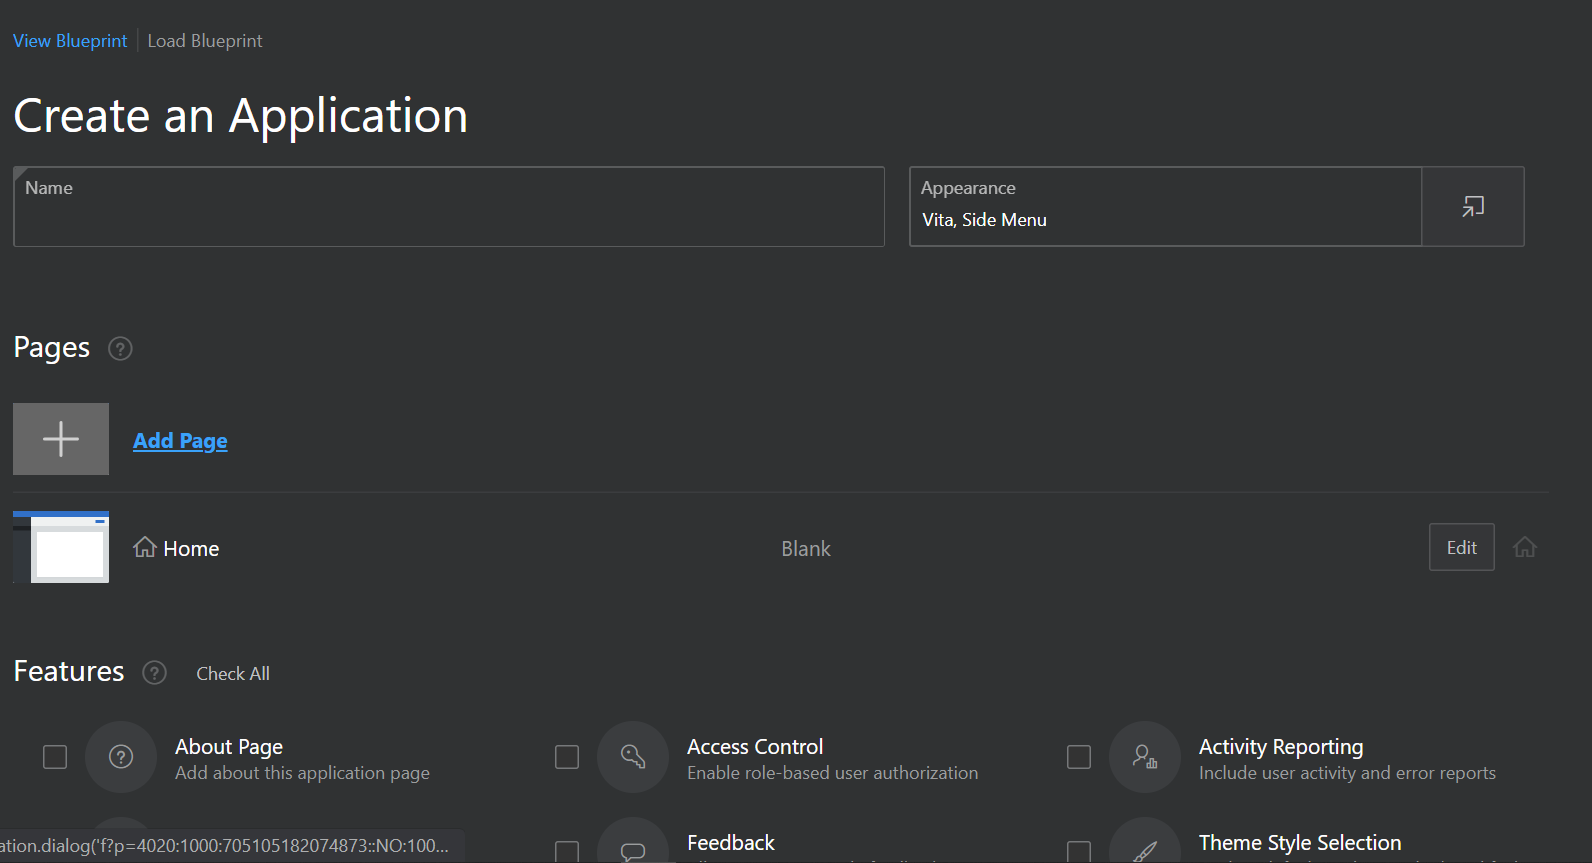
\includegraphics[width=9cm]{figures/12.png}
\end{figure}
\item Pada add page pilih "Interactive Report".
\begin{figure}[!htbp]
	\centering
	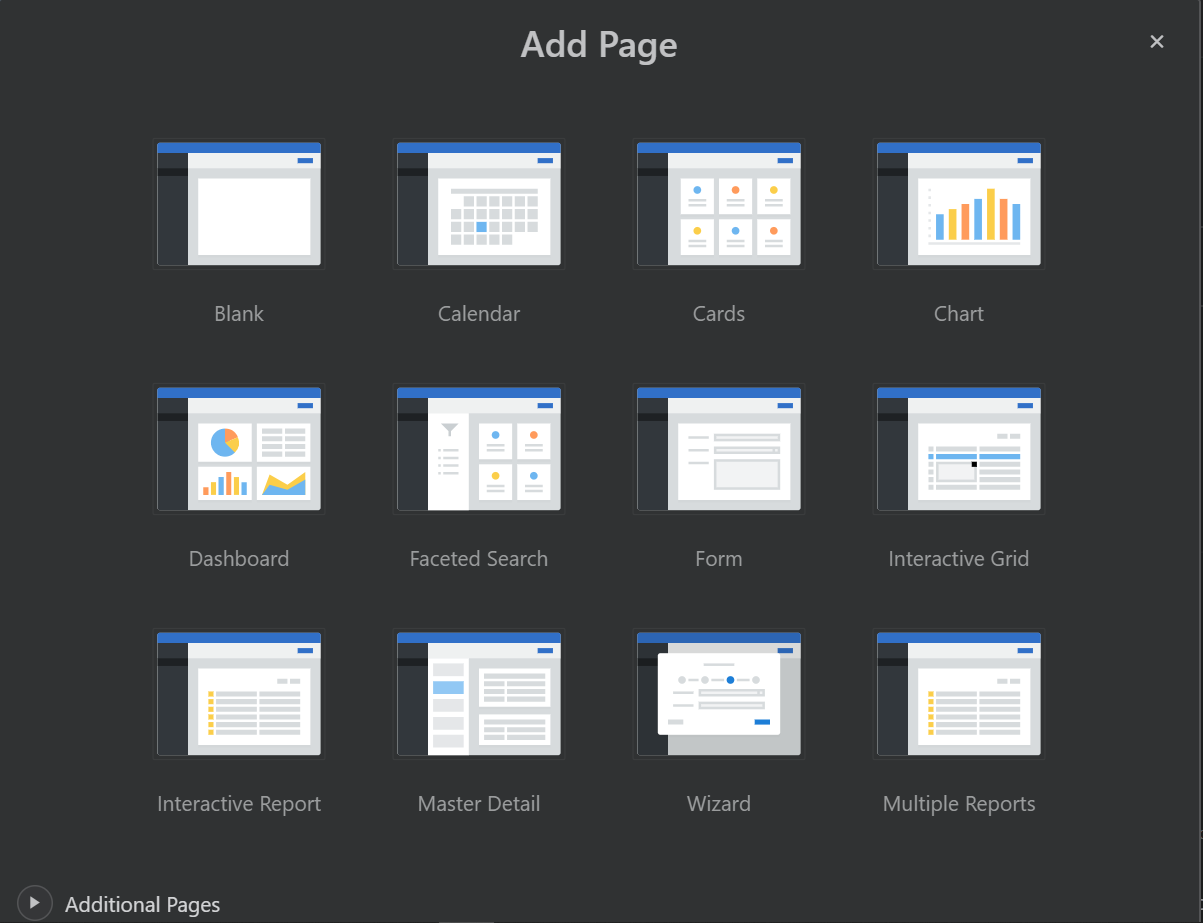
\includegraphics[width=10cm]{figures/13.png}
\end{figure}
\item Lalu kita mengisi form menu dan menambahkan tabel, klik pada tanda kotak merah di gambar untuk menambahkan tabel.
\begin{figure}[!htbp]
	\centering
	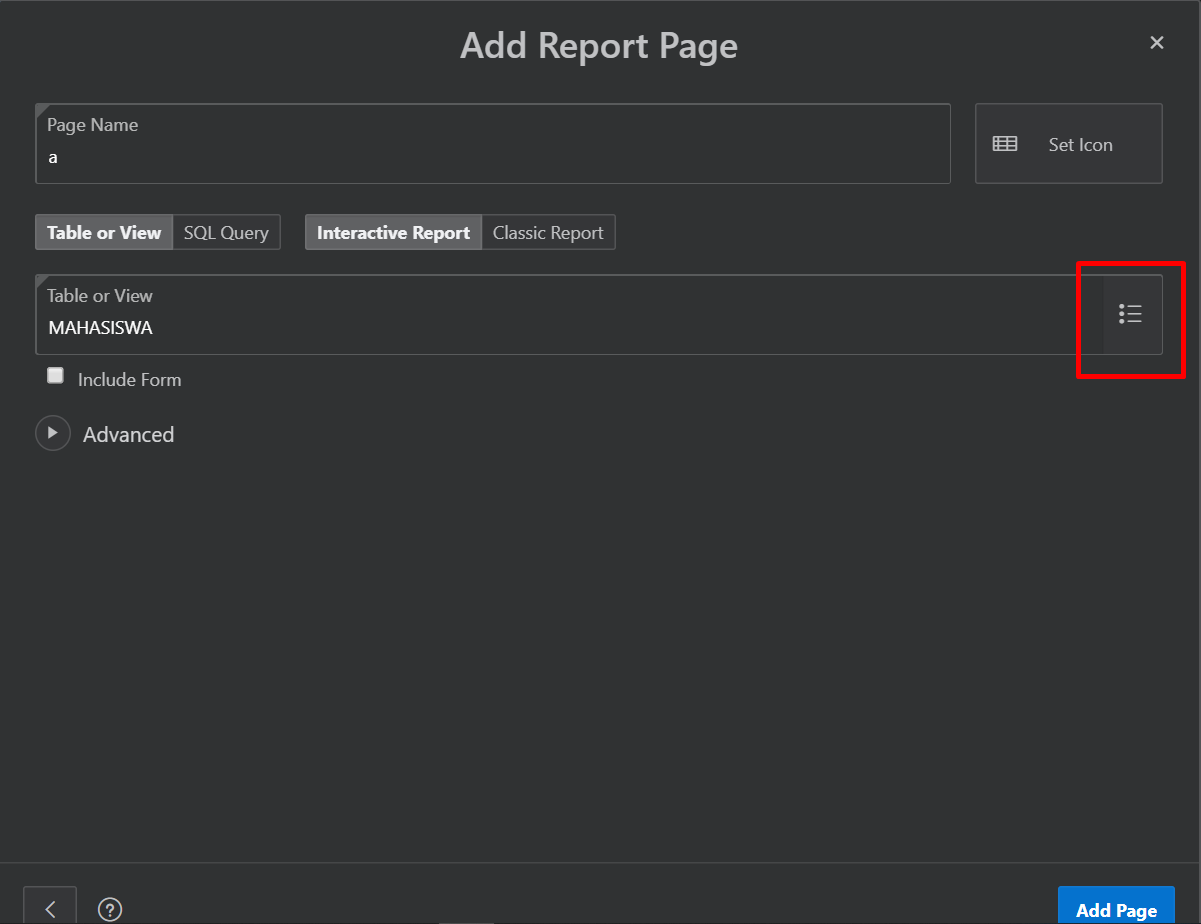
\includegraphics[width=10cm]{figures/14.png}
\end{figure}
\item Silahkan cari nama tabel mahasiswa, dan lakukan hal yang sama untuk tabel matkul, tabel nilaimhs, dan tabel logmhs.
\begin{figure}[!htbp]
	\centering
	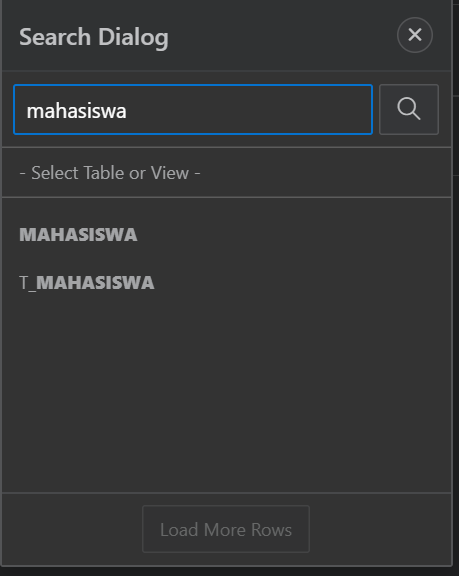
\includegraphics[width=6cm]{figures/15.png}
\end{figure}
\item Jika menu sudah ditambahkan sekarang tinggal menekan "Create Application" dan tunggu beberapa saat.
\item Setelah aplikasi dibuat jalankan aplikasi tersebut dengan klik "Run Application". Dan masuk dengan username dan password yang sama dengan waktu membuat workspace.
\begin{figure}[!htbp]
	\centering
	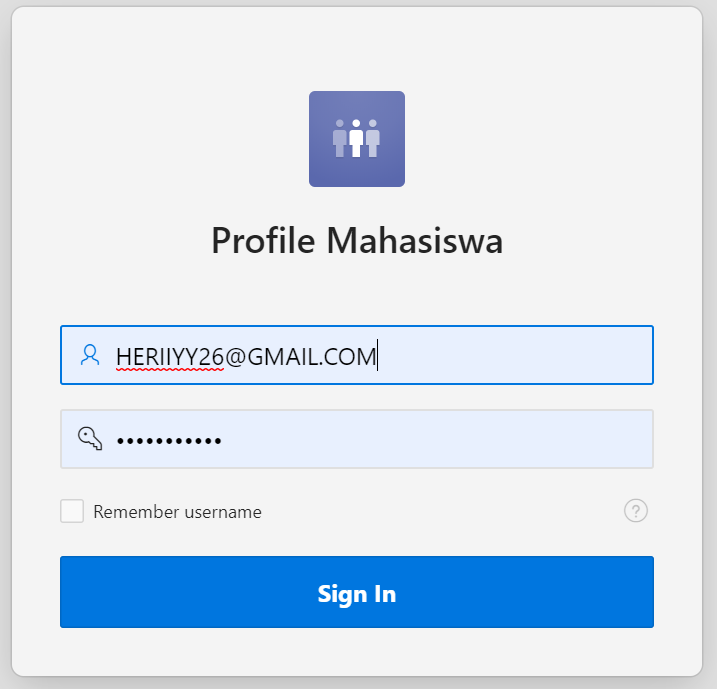
\includegraphics[width=6cm]{figures/28.png}
\end{figure}
\item Tampilan Dashboard Aplikasi.
\begin{figure}[!htbp]
	\centering
	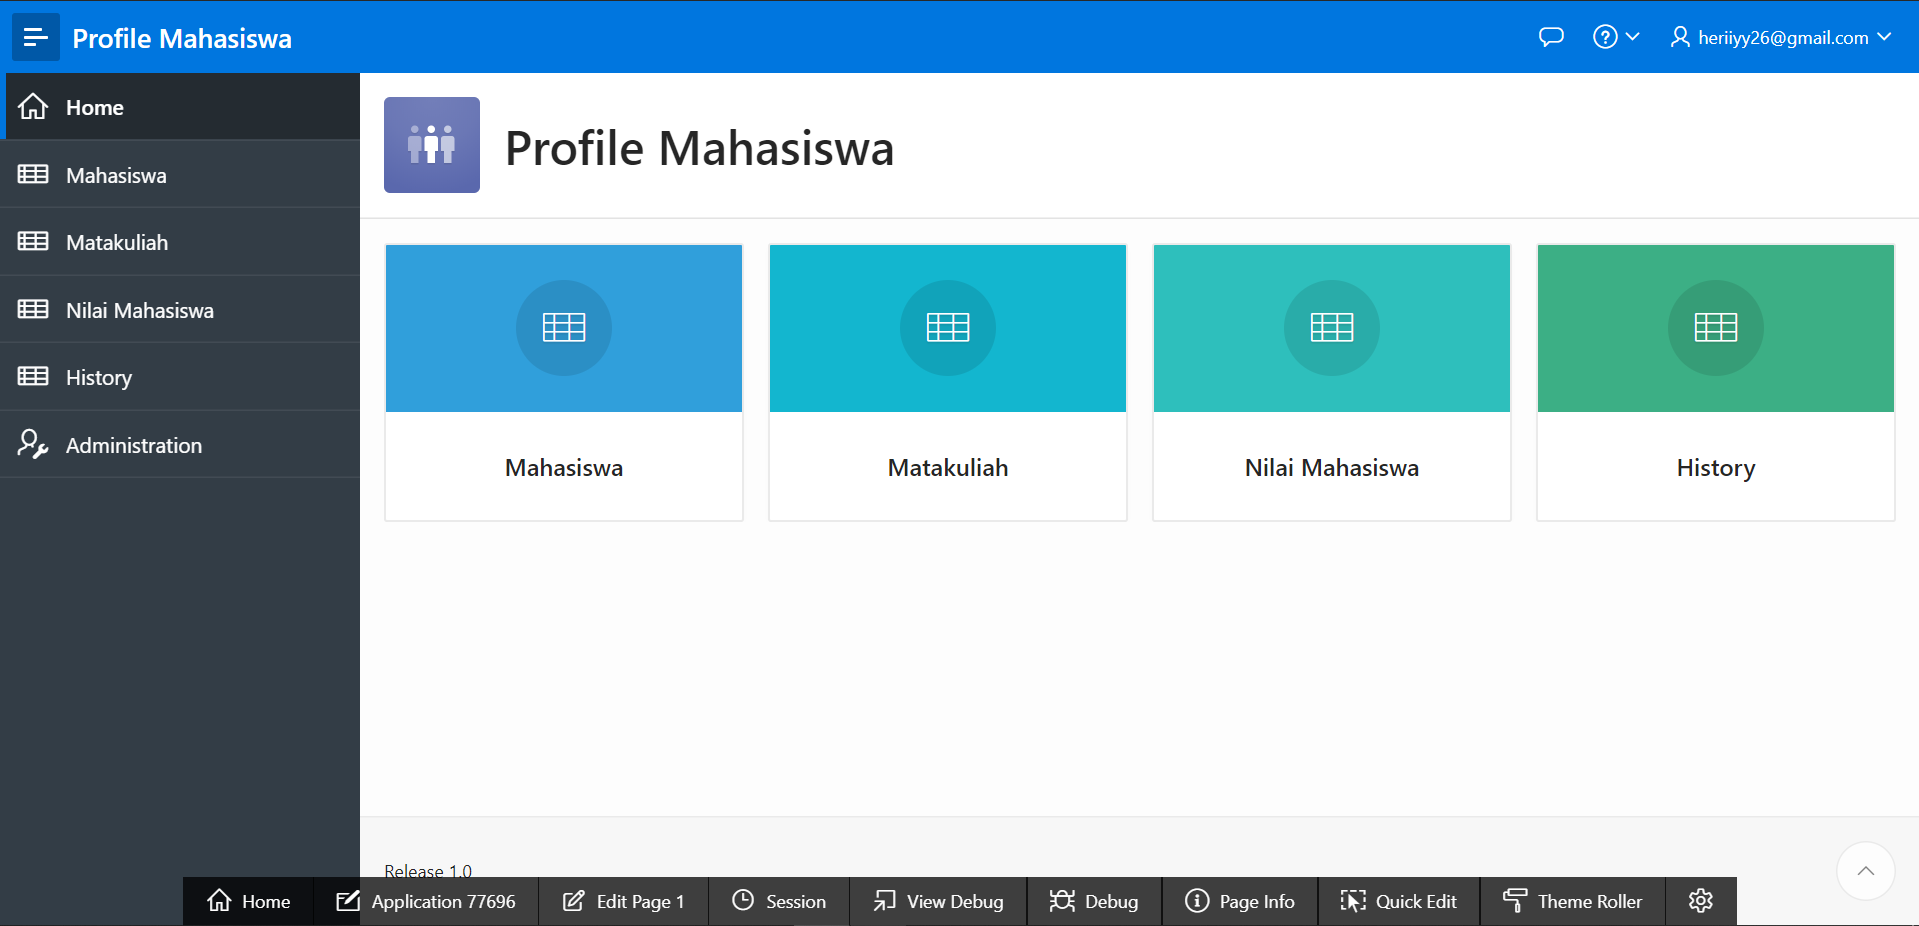
\includegraphics[width=12cm]{figures/29.png}
\end{figure}
\item Kita coba trigger after insert.
\begin{figure}[!htbp]
	\centering
	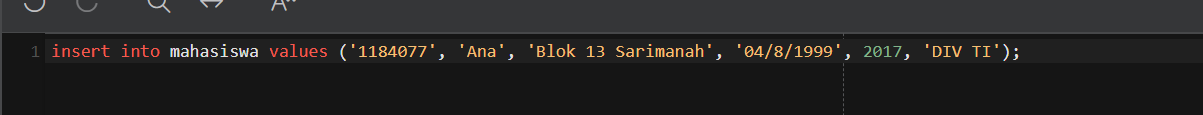
\includegraphics[width=13cm]{figures/23.png}
\end{figure}
\item Data berhasil dimasukkan otomatis.
\begin{figure}[!htbp]
	\centering
	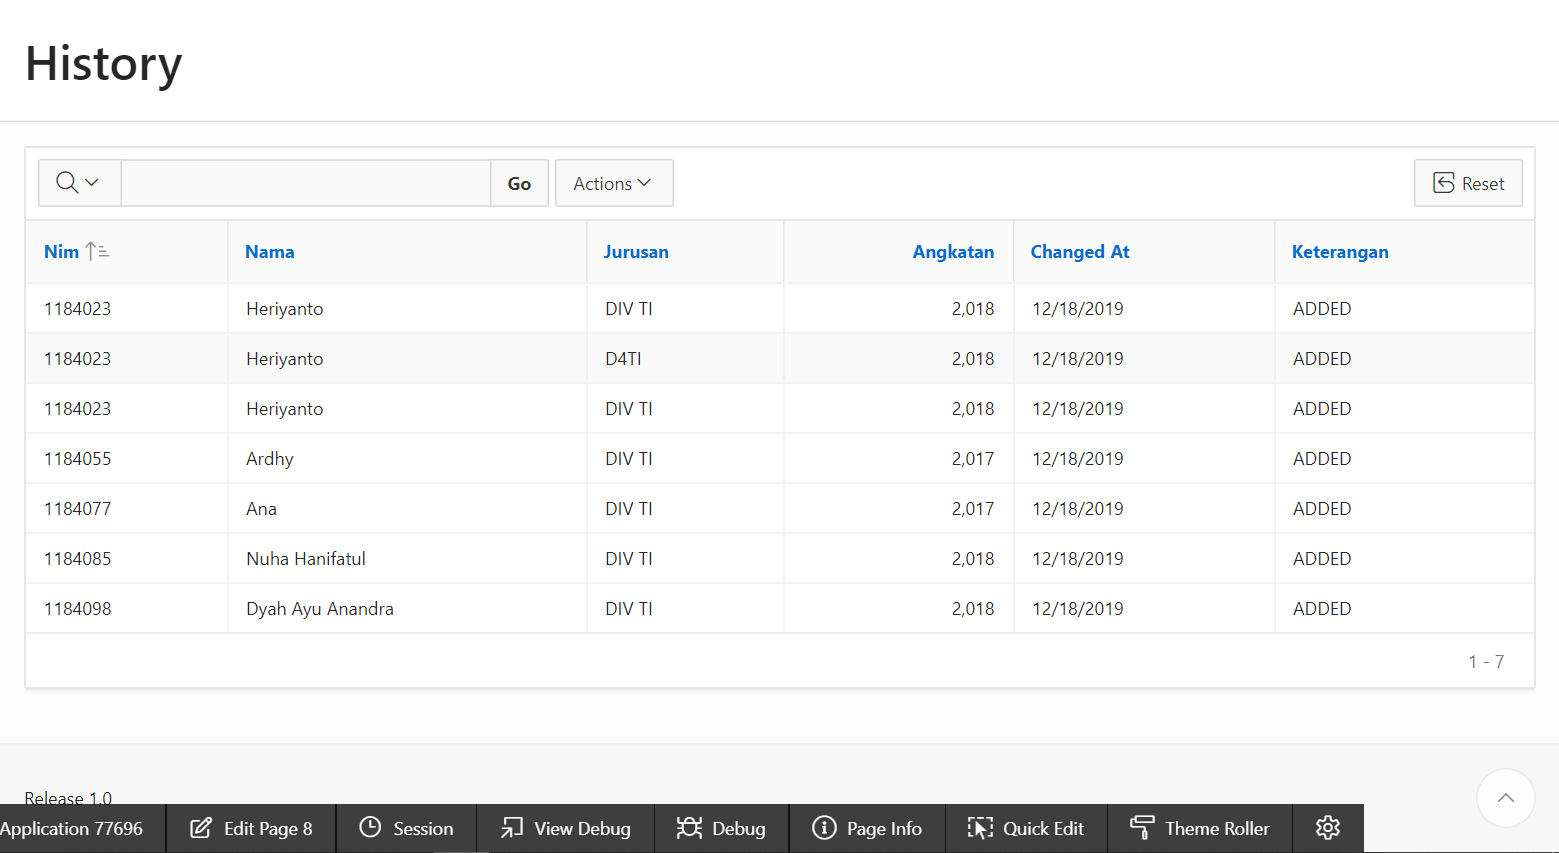
\includegraphics[width=12cm]{figures/24.png}
\end{figure}
\item Kita coba juga before insert.
\begin{figure}[!htbp]
	\centering
	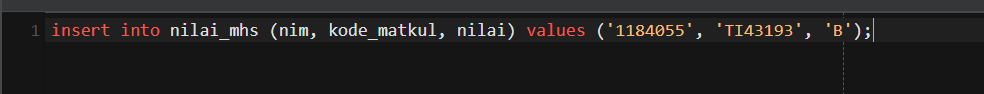
\includegraphics[width=10cm]{figures/25.png}
\end{figure}
\item Kolom tgl berhasil terisi otomatis berdasarkan waktu sekrang.
\begin{figure}[!htbp]
	\centering
	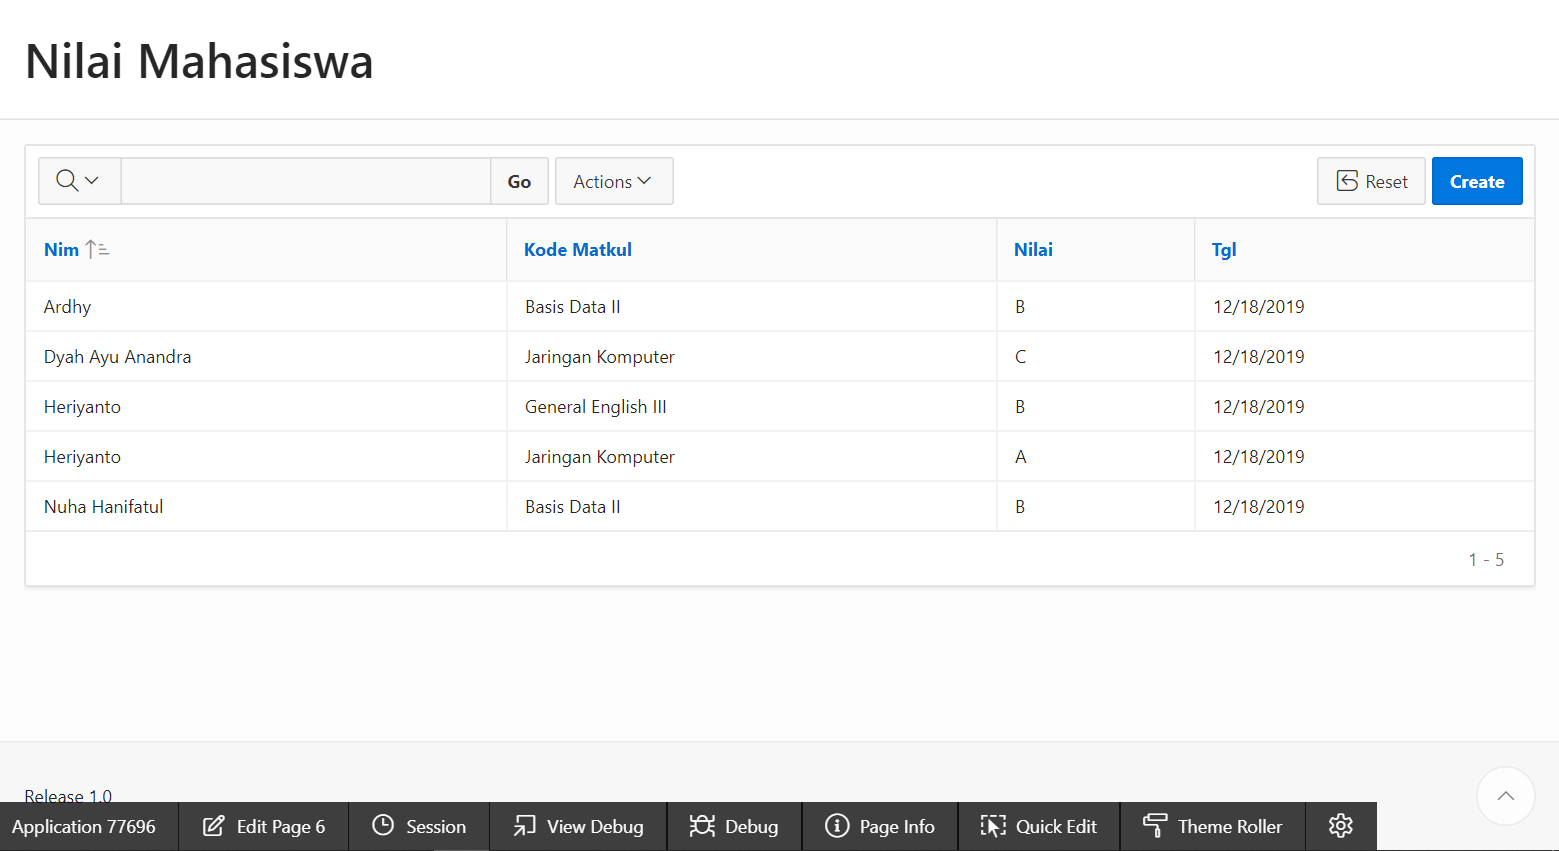
\includegraphics[width=10cm]{figures/26.png}
\end{figure}
\end{enumerate}
\section{Link}
\begin{enumerate}
\item Link = https://apex.oracle.com/pls/apex/f?p=77696:1:114506129892151:::::
\item ID = heriiyy26@gmail.com
\item PASS = makioshi194
\end{enumerate}
\end{document}